\documentclass[assign]{article}

\usepackage{graphicx}
\usepackage{amsmath,amssymb,amsthm} % define this before the line numbering.
\usepackage{color}
\usepackage{eso-pic}
\usepackage{bm}
\usepackage{caption}
\usepackage{epstopdf}
\usepackage{picins}
\usepackage[boxed]{algorithm2e}
\usepackage{url}
\usepackage{enumerate}
\usepackage{paralist}

% Declaring commonly used math operators
\DeclareMathOperator{\ddiag}{Diag}
\DeclareMathOperator{\rrank}{rank}
\DeclareMathOperator{\vvec}{vec}
\DeclareMathOperator{\tr}{tr}

\newcommand{\PhiB}{\mathbf{\Phi}}
\newcommand{\Ll}{\mathcal{L}}
\newcommand{\Nn}{\mathcal{N}}
\newcommand{\Uu}{\mathcal{U}}
\newcommand{\Ee}{\mathcal{E}}
\newcommand{\Aa}{\mathcal{A}}
\newcommand{\Hh}{\mathcal{H}}
\newcommand{\Ii}{\mathcal{I}}
\newcommand{\Ff}{\mathcal{F}}
\newcommand{\Dd}{\mathcal{D}}
\newcommand{\Tt}{\mathcal{T}}
\newcommand{\Pp}{\mathcal{P}}
\newcommand{\Ss}{\mathcal{S}}
\newcommand{\Cc}{\mathcal{C}}
\newcommand{\Oo}{\mathcal{O}}
\newcommand{\Bb}{\mathcal{B}}
\newcommand{\Rr}{\mathcal{R}}
\newcommand{\Rm}{\mathrm{R}}
\newcommand{\CB}{\mathbf{C}}
\newcommand{\RB}{\mathbf{R}}
\newcommand{\xB}{\mathbf{x}}
\newcommand{\yB}{\mathbf{y}}
\newcommand{\fB}{\mathbf{f}}
\newcommand{\ZB}{\mathbf{Z}}
\newcommand{\SB}{\mathbf{S}}
\newcommand{\AB}{\mathbf{A}}
\newcommand{\WB}{\mathbf{W}}
\newcommand{\TB}{\mathbf{T}}

\newcommand{\omitme}[1]{}
\newtheorem*{lemma}{Lemma}
\newtheorem{case}{Case}

\newenvironment{claim}[1]{\noindent\underline{{\bf Claim:}}\space#1}{}
\newenvironment{claimproof}[1]{\par\noindent\underline{{\bf Proof:}}\space#1}{\hfill$\square$}

\title{Homework 5}

\author{Prateep Mukherjee}

\begin{document}
\maketitle
1. We use a union-find data structure for this problem. As we know, the amortized cost of \emph{FIND} operation in union-find is $\mathcal{O}(\log n)$. We use the union-rank finding and the path-compression algorithms to reduce the amortized cost for find operation to $\mathcal{O}(\log n)$. Fig. \ref{fig1} shows an example of the data structure. The arrows denotes the edges from a child node to its parent node. The figure in the right shows the result of path-compression algorithm on the tree.

\begin{figure}[!hbt]
\centering
  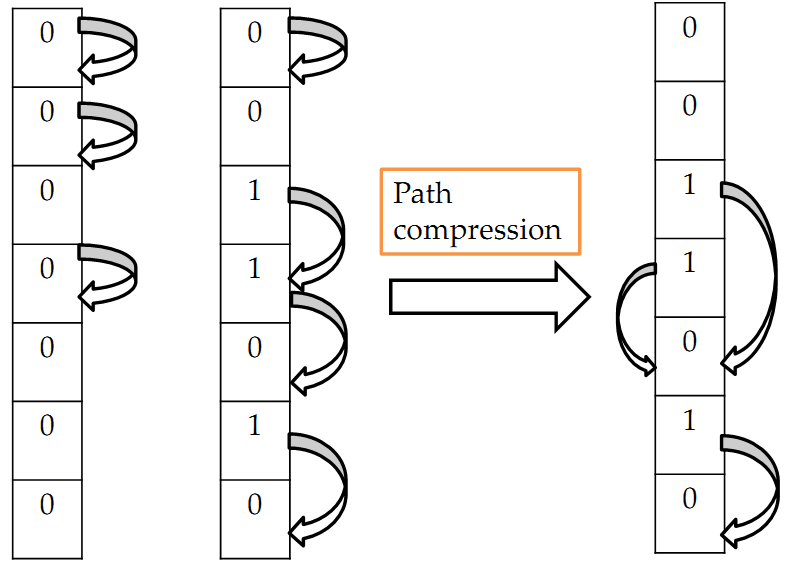
\includegraphics[width=0.9\linewidth]{fig1.png}
\caption{\small{ {\bf Left:} Initial array $A$ with all entries 0. Arrows indicate parent of each cell; {\bf Center:} Some of the entries set to 1. Notice that the arrows from each cell, containing 1, is directed to the next one; {\bf Right:} The path-compression algorithm redirects the arrows as shown, that is redirects the edges in the tree.}}
\label{fig1}
\end{figure}

Maintain an array $B$ where each element $B_i$ denotes the ancestor of element $i$. Initially, $B_i = i \forall i$

\begin{enumerate}[a.]
\addtolength{\itemsep}{-8pt}
\item \textbf{Set:} Set $A_i = 1$ and $B_i = i+1$
\item \textbf{Get:} Return $A_i$
\item \textbf{Find:} Use path-compression technique to find the nearest index $j \ge i$ s.t. $A_j = 0$. The algorithm for this can be written as:
\vspace{-5pt}
  \begin{algorithm}
      \caption{Find}
       \KwIn{$i$}
        \SetKwFunction{Find}{Find}
        \uIf{$A_i == 0$} {
             \KwRet{$i$}\;
         } 
	  \uIf {$i < length(A)$} {
             \KwRet{-1}\;
         } \Else {
              $B_i \gets \Find{$B_i$} $\;
             \KwRet{$B_i$}\;
         }
   \end{algorithm} 
\end{enumerate}

\begin{proof}[\textbf{Proof of correctness:}] Steps a and b is constant O(1). Since we are using the path-compression scheme in \textsc{Find}, the amortized cost is $\mathcal{O}(\log n)$, as we are moving up to the root of the tree.
\end{proof}

\vspace{10pt}

\par 2. {\bf 6 is the lower bound} for the number of questions asked. A \textbf{decision tree} can be used to generate the output. In the decision tree, answer yes points to the right, and answer no points to the left. Now, in a decision tree, each question asked depends on the previous answer, each time dividing the search space at the parent node into half. Height of the decision tree is $\mathcal{O} (\log 64) = 6$, as there are 64 possible outputs and hence at least 64 possible leaves.

\par {\bf 6 is also the upper bound} for this problem. This is because we can represent each number from 1 to 64 using at most 6 bits. Any more bits used will be redundant. Therefore, a tight upper bound should be 6, as one need not ask any more than 6 yes/no questions to get the optimal answer. 

\par Since information-theoretic upper and lower bounds for this problem is the same, the decision tree model for answering the question is optimal.

\vspace{10pt}

\par 3. (a) Let, set $Y = \{000, 001, 110, 111\}$. This set is fixed. Now, by only looking at the first 2 bits of an input string, we can say if the string exists in set Y. This is because the possibilities for string s is $\{00X, 11X, 10X, 01X\}$, where $X$ denotes the dont-care character. Now, if the adversary gives us a string from the first 2 strings, we can directly say that it exists in set Y. On the other hand, if a string is given from the last 2 strings, we can directly say it doesn't exist in Y.

\par (b) We prove this using the principle of induction. Let, $n$ be the length of strings in Y as well as the input string s, and $L$ be the cardinality of set Y. It is given that $L$ is odd.

\par \textbf{Base case:} Consider $n=1$. Now, since $L$ is odd, set Y will either have the bit 0 or 1. Therefore we need to read the one and only bit of string s to ensure if it lies(or not) in set Y. 
\par Similarly, if $n=2$, set Y can contain only 1 or 3 possible strings. So, if the adversary selects a string which does not exist in Y, however the first bit matches with some string in Y, then our algorithm fails. Therefore, we have to check all the bits in string s to ensure it does(or not) lie in Y.

\par \textbf{Inductive case:} Assume we have proved the problem for $n=k$. When $n = k+1$, since the number of strings in Y is odd, at least one string in Y will contain exactly the same $n-1$ bits as that of s. 
\par Therefore, if we do not look at the $n^{th}$ bit of string s, then the adversary might replace the above matched string, but with the last bit flipped. 

This proves that we need to look at all the bits of string s, if set Y has odd number of strings.

\vspace{10pt}

\par 4. (a) The \textsc{BoxDepth} problem can be reduced to \textsc{MaxClique} as follows:
\vspace{-5pt}
\begin{itemize}
  \addtolength{\itemsep}{-8pt}
  \item Create a graph $G$ where every node denotes a rectangle.
   \item For each pair of rectangles $(i,j)$, if they have a non-zero intersection area, connect nodes $i$ and $j$ in $G$.
   \item Solving the \textsc{MaxClique} problem on $G$ gives us the largest subset of intersection of the rectangles.
\end{itemize}

\begin{proof}[\textbf{Proof of correctness:}]
  The reduction has polynomial-time complexity as we are iterating over every pair of nodes, that is $\mathcal{O}(n^2)$.
\end{proof}

\par (b) The \textsc{BoxDepth} problem can be solved in polynomial time using $\mathcal{O}(n^3)$ algorithm as follows:

\begin{algorithm}[H]
   \caption{BoxDepth}
    \KwIn{List of $n$ axis-aligned(say Y-axis) rectangles}
    \KwOut{number of largest subset of intersection of them}
    \SetKwFunction{sort}{sort}
    $\sort{List  wrt  X-interval}$\;
    $L \gets \emptyset$\;
    $res \gets 0$\;
     \For{ each rect $i$}  {
         \For{ every other rect $j$} {
              $X \gets interval \; of \; intersection \; of \; rectangles \; i \; \& \; j$\;
              $L \gets L \cup X$
          }
      }
      \For{each $l \in L$} {
           $count \gets number \; of \; rectangles \; containing \; interval \; l$\;
	    $res \gets \max{(count,res)}$\;
       }
       \KwRet{res}
\label{algo1}
\end{algorithm}

The algorithm \ref{algo1} reduces the 2D problem to 1D problem of finding intervals. In the two nested for loops at the beginning, we find the list of intersections(in X-direction) for all the rectangles. In the final for loop, for each X-interval we look at all the other rectangles it overlaps with and update the count. The rectangles are sorted wrt X-interval in the beginning, so a forward update would work.
 \vspace{-5pt}
\begin{proof}[\textbf{Proof of correctness:}]
Sorting $n$ rectangles initially takes $\mathcal{O}(n\log n)$ using quicksort. The nested for loop in the beginning takes $\mathcal{O}(n^2)$ to compute the list of X-intervals. The final loop iterates over each rectangle for each interval. Thus, the total time complexity is $\mathcal{O}(n^3)$.
\end{proof}

\par \noindent (c) In the previous section we proved a polynomial time algorithm for \textsc{BoxDepth}. To show P=NP, that is to show that \textsc{BoxDepth} is NP-hard, we need to show that a known NP-hard problem(e.g. \textsc{MaxClique}) can be reduced to \textsc{BoxDepth}. In the first part, however, we proved the reverse. Therefore, the above two solutions do not prove that P=NP.

\vspace{10pt}

\par 5. Let, $OPT$ be the optimal makespan of scheduling jobs on $m$ machines. Also, let $T_i$ be the time required to execute a job $i$ and $Total_k$ be the total time that a machine $k$ is busy using the greedy assignment strategy.  Let, $i$ be the busiest machine and $j$ be the last job assigned to it. So, machine $i$ had the optimal makespan before the last job was added. Therefore, we can write:

\begin{eqnarray}
&  Total_i - T_j  \le Total_k \label{l1} \\
 & \implies  m(Total_i- T_j) \le \sum_{i=1}^{m} Total_i \; \; \;  \label{l2}  \\
 & \implies Total_i - T_j \le 1/m \times \sum_{i=1}^{n} T_i \le OPT \label{l3} 
\end{eqnarray}

Eqn \ref{l1} simply denotes the claim above. We get eqn \ref{l2} by summing eqn \ref{l1} $m$ times. The term on the right in eqn \ref{l2} is the sum of the execution times for all the machines, which is equal to the sum total of execution for all the jobs. Thus, we can replace machines with jobs in eqn \ref{l3}. This is clearly less than $OPT$ as the latter is maximum of busiest times for all the machines. 

\par Also, $\forall i \; \; T_i \le OPT$ as the optimal makespan must include the longest job. Putting this and eqn. (\ref{l3}) together, we get the following:

\begin{equation*}
   Total_i \le 2 \cdot OPT, \forall i
\end{equation*}

To obtain a stricter upper bound, let us assume we schedule $n = m(m-1)+1$ jobs onto $m$ machines. Let, the first $n-1$ jobs have execution times of 1, i.e. $T_i = 1, i \in \left [1,n-1\right ]$ and the last job $n$ has execution time of m, i.e. $T_n = m$.  The optimal assignment schedules $n-1 = m(m-1)$ jobs onto $m-1$ machines and the last job onto a machine, with no other jobs on it. Thus, $OPT = m$. Using the greedy strategy, however, before the last job arrives, $n-1$ jobs are schedules onto $m$ machines, with makespan = $m-1$. After the last job,  makespan = $m-1+m = 2m-1$. Thus the ratio of greedy to optimal is $\frac{2m-1}{m} = 2 - 1/m$. 

\begin{equation}
  \nabla \lambda = \begin{bmatrix}
 G^{a}_{p} \\
 G^{b}_{p} \\
 G^{c}_{p} 
\end{bmatrix}
\end{equation}

\begin{equation}
  \hat{n}^{k}_{i}
\end{equation}


\end{document}